\question 下列关于定点数原码一位乘算法的描述正确的是( )。
Ⅰ.符号位不参加运算,根据数值位的乘法运算结果确定结果的符号位
Ⅱ.在原码一位乘算法过程中,所有移位均是算术移位操作
Ⅲ.假设两个n位数进行原码一位乘,部分积至少需要使用n位寄存器
\par\twoch{Ⅱ、Ⅲ}{只有Ⅱ}{只有Ⅲ}{\textcolor{red}{全错}}
\begin{solution}Ⅰ:在原码一位乘中,符号位是不参加运算的,结果的符号位是被乘数的符号位和乘数的符号位``异或''的结果,故Ⅰ错误。
Ⅱ:在原码一位乘算法中,由于参与操作的数是真值的绝对值,因此没有正负可言,故在原码一位乘法中运算过程中所有的移位均是逻辑移位操作,即在高位添加0,故Ⅱ错误。
Ⅲ:由于在部分积相加中,可能导致两个小数相加大于1,因此部分积至少需要使用n+1位寄存器,故Ⅲ错误。
综上所述,Ⅰ、Ⅱ、Ⅲ全错。
\end{solution}
\question 假设机器字长为16位,用定点补码小数表示时,一个字所能表示的范围是
\par\fourch{}{}{}{\textcolor{red}{}}
\begin{solution}D。
在小数定点机中,如果采用补码表示,则0的编码是唯一的,因此补码可以比原码和反码多表示一个-1,至于为什么,已经在前面知识点中很详细地讲解过了。另外,假设机器字长为n位,不管原码、补码、反码,上限都是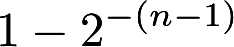
\includegraphics[width=0.83333in,height=0.17708in]{texmath/8dff4c5Cdpi7B3507D1-7B25E7B-28n-1297D7D}。
\end{solution}
\question 计算机运算溢出检测机制,采用双符号位,下列关于双符号位的说法中正确的有(
) I. 00表示正号,11表示负号
II.结果的符号位为01时,称为上溢;为10时,称为下溢
III.符号位都为00的两个数相加,运算结果有可能产生溢出
IV.符号位都为11的两个数相加,运算结果不会产生溢出
\par\twoch{I}{I、II和IV}{I和IV}{\textcolor{red}{I、II和III}}
\begin{solution}I明显正确,这是规定。
II这个我们可以举例进行检验,比如举个上溢的例子,两个比较大的正整数相加,如00
1100 + 00 1100 = 01 1000。还可以举个下溢的例子,故II正确。
III正确,当两个同符号的数相加(或者是相异符号数相减)时,运算结果有可能产生溢出。
IV错误,解释如上。 故本题选D。
\end{solution}
\question 下列关于溢出的说法中,正确的是
\par\fourch{正数和负数相加,如果结果为负数(符号位为 1),表明发生溢出}{\textcolor{red}{两个负数相加,如果结果为正数(符号位为 0),表明发生溢出}}{浮点数的溢出与否由尾数的符号决定,比如[尾数]补=01,××…×为上溢}{全错}
\begin{solution}B。 A错误,正数和负数相加不会产生溢出。 B正确。
C错误,当尾数出现01,××\ldots{}×或10,××\ldots{}×时,表示尾数溢出,这在定点加减运算中是不允许的,但在浮点运算中这不算溢出,可通过右规处理。右规时尾数右移一位,阶码加1。所以浮点机的溢出与否不是由尾数的符号位决定的,它是由阶码的符号决定,即{[}阶码{]}补=01,××\ldots{}×为上溢,需作溢出处理,{[}阶码{]}补=10,××\ldots{}×为下溢,按机器零处理。
\end{solution}
\question 设机器数采用移码表示(含1位符号位),若寄存器内容为9BH,则对应的十进制数为
\par\twoch{\textcolor{red}{27}}{-97}{-101}{155}
\begin{solution}A。
同一个数的补码与移码只相差一个符号位,移码9BH=
\includegraphics[width=0.86458in,height=0.18750in]{texmath/c89dca5Cdpi7B3507D281001+101129_2},同一个数的补码为0001
1011,即27。
\end{solution}
\question 若采用双符号位,则两个正数相加产生溢出的特征时,双符号位为
\par\twoch{00}{\textcolor{red}{01}}{10}{11}
\begin{solution}B。
采用双符号位时,第一符号位表示最终结果的符号,第二符号位表示运算结果是否溢出。若第二位和第一位符号相同,则未溢出;不同,则溢出。若发生正溢出,则双符号位为01;若发生负溢出,则双符号位为10。
如考生临时忘记,可用自己举例求证。这里举双符号位,双数值位的特例。
如3+3的情况,(00 11)补+(00 11)补=(01 10)补。正溢出。
如(-3)+(-3)的情况,(11 01)补+(11 01)补=(10 10)补。负溢出。
\end{solution}
\question 某机字长16位,其中包括1位符号位。用定点补码表示小数时,一个字能表示的范围是
\par\twoch{0~(1-$2^-15$)}{-(1-$2^-15$)~(1-$2^-15$)}{-1~1}{\textcolor{red}{$-1~(1-2^-15$)}}
\begin{solution}D。 字长16位,除去1位符号位,数值位15位,最小负数为1.000 0000 0000
0000,即-1,最大正数为0.111 1111 1111,即(1-$2\^{}-15$)。
\end{solution}
\question 关于下列三段代码说法正确的是 int max(int a,int b) \{
if(a-b\textgreater{}0) return a; else return b; \} int max(int a,int b)
\{ if(a\textgreater{}b) return a; else return b; \} int max(int a,int b)
\{ if(-a\textless{}-b) return a; else return b; \}
\par\twoch{三段代码都是正确的}{有两段是正确的,一段是错误的}{\textcolor{red}{有一段是正确的,其余都是错误的}}{三段代码都有错误}
\begin{solution}C。
第一段是错误的,两个int型变量相减可能产生溢出,所以程序员和编译器不能用表达式(a-b大于0)来代替(a大于b)。甚至于也不能用表达式(-b小于-a)来替换,因为在二进制补码表示中负数和正数的范围是不对称的,所以第三段也是错误的。只有第二段才是正确的代码。
\end{solution}
\question 设机器数字长为8位(含1位符号位在内),若{[}x{]}补={[}x{]}原,则x的真值的取指范围为
\par\twoch{x大于0}{x≥0}{\textcolor{red}{x≥0和x=-1/2}}{x=0}
\begin{solution}C。 若x≥0,原码跟补码一样。
若x小于0,当x=-1/2时,补码和原码都是1.1000000。故选C。
\end{solution}
\question 下面的代码是一个C语言函数,用来计算两个长为len(len小于1000)的数组a和数组b对应元素的和,结果保存在数组c中,其中c{[}i{]}=a{[}i{]}+b{[}i{]}。当len为0时,返回值应该是空数组,但在执行时,却提示``Runtime
Error:Segmentation
fault''。后经检查是一个语句有误,改后就正常执行了。这个语句可能是 double
*sum\_array(double A{[}{]},double B{[}{]},unsigned int len) //① \{ int
i; //② double C{[}1000{]}; //③ for(i=0;i小于等于len-1;i++) //④ C{[}i{]}
= A{[}i{]}+B{[}i{]}; //⑤ return C; //⑥ \}
\par\twoch{①}{③}{④}{\textcolor{red}{①或④}}
\begin{solution}D。 Segmentation
fault,段错误就是访问了错误的内存段,一般是你没有权限,或者根本就不存在对应的物理内存。内存访问异常是由于对数组A,B访问时产生了越界错误而造成的。循环变量是int型的,而len是unsigned
int型,当len为0时,执行len-1的结果为FFFF
FFFF,是最大的可表示的32位无符号数,任何无符号数都比它小,使得数组越界访问,因而发生Segmentation
fault。 可以通过修改参数len的声明为int型,就能避免这一错误。
也可以将for(i=0;i小于等于len-1;i++)中的i小于等于len-1改为i
\end{solution}
\question 一个C语言程序在一台32位机器上运行,定义了两个变量x,y,其中x的数据类型为int、y的数据类型为float。已知x=2013,y=201.3,则在一个32位机器中执行下列表达式时,结果为``真''的有
I.x==(int)(float)x II.y==(float)(int)y III.y==(float)(double)y
\par\twoch{I}{I和II}{II和III}{\textcolor{red}{I和III}}
\begin{solution}D。
C语言算术表达式的计算,在计算过程中,每一步计算所得结果的数据类型由参与运算的运算对象决定,相同数据类型的两个对象运算,结果数据类型不变,不同数据类型的运算对象进行运算,结果的数据类型由高精度的运算对象决定。精度的高低:double大于float大于int。
本题中强制类型转换,从精度低的数据类型转换为精度高的数据类型,不会发生溢出,反之就会发生溢出,如从double或float转换为int时,小数部分被截断。
故本题I中,int类型的x转换为float后没有发生溢出,且没有发生数据舍入。再由float类型转换为int类型,也保留了x原来的值2013,故I正确。
本题II中,float类型的y转换为int后,小数部分被截断,值为201。再转换为float类型后值还是为201,与201.3不等,故II错误。
本题III中,float类型的y转换为double后,值还是为201.3。再转换为double类型后值还是为201.3,故III正确。
综上,本题选D。
\end{solution}
\question 考虑以下C语言代码: short si =-8196; int i = si;
执行上述程序段后,i的机器数表示为
\par\twoch{0000 9FFCH}{0000 DFFCH}{FFFF 9FFCH}{\textcolor{red}{FFFF DFFCH}}
\begin{solution}D。 解法一: 求出si的16位补码,扩展成32位。 si的16位补码为1101 1111 1111
1100,扩展为32位为 1111 1111 1111 1111 1101 1111 1111 1100,即为FFFF
DFFCH。 解法二: 可知i=si=-8196,直接求-8196的32补码。
-8196的32位补码为1111 1111 1111 1111 1101 1111 1111 1100,即为FFFF
DFFCH。 【总结】很明显解法二更直接,将问题简化了。
\end{solution}
\question 考虑下列C语言程序代码: int i=65535; short si=short(i); int j = si;
假定上述程序段在某32位机器上执行,sizeof(int)=4,则变量i、si和j的值分别是
\par\fourch{65535、65535、65535}{65535、1、-1}{\textcolor{red}{65535、-1、-1}}{65535、-1、1}
\begin{solution}C。
在一台32位机器上执行上述代码段时,i为32位补码表示的定点整数,第2行要求强行将一个32位带符号数截断为16位带符号整数,65535的32位补码表示为0000
FFFFH,截断为16位后变成FFFFH,在16位补码表示中,它表示-1,因此si的值为-1。
再将该16位带符号整数扩展(扩展不能改变数值大小,即j还应该是-1)为32位时,就变成了FFFF
FFFFH。因此j的值也为-1。 综上,本题选择C。
\end{solution}
\question 当定点运算发生溢出时,应
\par\twoch{向左规格化}{向右规格化}{舍入处理}{\textcolor{red}{发出出错信息}}
\begin{solution}D。
定点数运算如果发生溢出,则必须发出出错信息进行中断处理,不要和浮点数的尾数溢出混淆。
\end{solution}
\question 下列关于定点数一位原码乘法的描述正确的是
Ⅰ.符号位不参加运算,根据数值位的乘法运算结果确定结果的符号位
Ⅱ.在原码一位乘算法过程中,所有的移位均是算术移位操作
Ⅲ.假设两个n位数进行原码一位乘,部分积至少需要使用n位寄存器
\par\twoch{Ⅱ、Ⅲ}{只有Ⅱ}{只有Ⅲ}{\textcolor{red}{全错}}
\begin{solution}D。
Ⅰ:在原码一位乘中,符号位是不参加运算的,结果的符号位是被乘数的符号位和乘数的符号位``异或''的结果,故Ⅰ错误。
Ⅱ:在原码一位乘算法中,由于参与操作的数是真值的绝对值,所以没有正负可言,故在原码一位乘法中运算过程中所有的移位均是逻辑移位操作,即在高位添加0,故Ⅱ错误。
Ⅲ:由于在部分积相加中,可能导致两个小数相加大于1,所以部分积至少需要使用n+1位寄存器,故Ⅲ错误。
综上所述,Ⅰ、Ⅱ、Ⅲ全错。
\end{solution}
\question 在原码两位乘中,符号位单独处理,参加操作的数是
\par\twoch{原码}{\textcolor{red}{绝对值的补码}}{补码}{绝对值}
\begin{solution}B。
此题属于概念题,在前面知识点讲解的过程中,多次强调原码乘法采用的是绝对值的补码。
\end{solution}
\question 假设机器字长为8位(含两位符号位),若机器数DAH为补码,则算术左移一位和算术右移一位分别得
\par\twoch{\textcolor{red}{B4H  EDH}}{F4H  6DH}{B5H  EDH}{B4H  6DH}
\begin{solution}A。
首先先将机器数DAH表示成二进制,即11011010,在前面知识点讲解中,提过两位符号位的算术移位思想,即高位符号位不参与移位,低位符号位需要参与移位,算术左移变成10110100(补码算术左移,低位补0),转成十六进制,即B4H;算术右移变成11101101(补码算术右移,高位添加符号位,此题应该补1),转成十进制,即EDH。
\end{solution}
\question 下列关于各种移位的说法中正确的是
Ⅰ.假设机器数采用反码表示,当机器数为负时,左移时最高数位丢0,结果出错;右移时最低数位丢0,影响精度
Ⅱ.在算术移位的情况下,补码左移的前提条件是其原最高有效位与原符号位要相同
Ⅲ.在算术移位的情况下,双符号位的移位操作中只有低符号位需要参加移位操作
\par\twoch{Ⅰ、Ⅲ}{只有Ⅱ}{只有Ⅲ}{\textcolor{red}{Ⅰ、Ⅱ、Ⅲ}}
\begin{solution}D。 Ⅰ和Ⅱ看前面的总结,故Ⅰ、Ⅱ都是正确的。
Ⅲ:为了防止左移操作造成溢出,补码的算术左移需要一个前提条件,即其原最高有效位需要与符号位相同。对于这句话的理解,使用两位符号位更为方便。正常情况下,采用两位符号位时,符号位为00或11表示正常。如果最高数值位和符号位不一样,则左移就会导致符号位为10或者01,造成溢出。
综上所述,Ⅰ、Ⅱ、Ⅲ都是正确的,故选D。
\end{solution}
\question 补码定点整数1101 0000右移两位后的值为
\par\twoch{0100 0000}{0011 0100}{\textcolor{red}{1111 0100}}{都错}
\begin{solution}C。 本题类似上题,希望大家练习用方法二试着解题,举一反三。
解法一:该数为补码,符号位为1,按照算术补码移位规则,负数右移添1,负数左移添0,所以1101
0000右移两位后为1111 0100。 解法二:右移就是除以4。补码1101
0000,原码为1011
0000,十进制数为-(2\^{}5+2\^{}4),除以4后为-(2\^{}3+2\^{}2),原码为1000
1100,补码为1111 0100。
【注意】所有移位操作的题目,都可以化成十进制进行求解或验算。左移n位相当于对应的十进制数×2\^{}n,右移n位相当于对应的十进制数×2\^{}(-n)。
\end{solution}
\question 下列关于各种移位的说法正确的是
Ⅰ.假设机器数采用反码表示,当机器数为负时,左移时最高数位丢0,结果出错;右移时最低数位丢0,影响精度
Ⅱ.对于变形补码,在算术移位的情况下,补码左移的前提条件是其原最高有效位与原符号位要相同
Ⅲ.在算术移位的情况下,双符号位的移位操作只有低位符号位需要参加移位操作
\par\twoch{Ⅰ、Ⅲ}{只有Ⅱ}{只有Ⅲ}{\textcolor{red}{Ⅰ、Ⅱ和Ⅲ}}
\begin{solution}D。 Ⅰ:看下面的总结,故Ⅰ正确;
Ⅱ:正常情况下,变形补码的符号为00或者11时不溢出,如果最高有效位与原符号位不同,比如11.0XXX,左移就会形成10.XXX这种形式,导致溢出,故Ⅱ正确;
Ⅲ:看下面的总结,故Ⅲ正确。
总结:原码、补码、反码哪种情况的移动影响精度,哪种情况下的移动结果出错?
解析:首先,对于正常的一个数来讲,高位上的权重是肯定比低位上的权重要大很多,前面我们讲过8位机器字长拿出一位作为符号位,其最大值立马减少一半,说明如果高位丢失了,结果就会出错。而低位丢失了仅仅是影响精度而已。上面说的很清楚,对于一个正常的真值来说,而在原码、补码、反码中只有原码是和真值的数值位一样的,所以说得出以下结论:
(1)对于正数,原码、补码、反码的数值位都是和真值一样的,都属于正常数,所以机器数为正时,左移时最高数位丢1,结果出错;右移时最低数位丢1,影响精度。
(2)对于负数,需要分以下3种情况:
原码:不管是正数还是负数,原码的数值位永远和真值是一样的,所以仍然是左移时最高数位丢1,结果出错;右移时最低数位丢1,影响精度。
反码:当机器数为负数时,反码的数值位和原码恰好相反,所以原码丢1,对应反码丢0才对,故应该为:左移时最高数位丢0,结果出错;右移时最低数位丢0,影响精度。
补码:补码就更简单了,右移丢低位和原码一样,左移丢高位和反码一样,故应该为:右移时最低数位丢1,影响精度;左移时最高数位丢0,结果出错;
最后还有一个很多教材没有涉及的重中之重的双符号位的算术移位,记住一个结论,这个结论在溢出也会讲到,这个结论是如果采用双符号位来表示数,永远是最高符号位才是真正的符号位。所以在算术移位的时候只有高符号位保留不变,低符号位是要参与移位的。
例如:11.110011(采用双符号位,假设采用补码表示),那么算术左移一位和算术右移一位分别是11.100110和11.111001。
\end{solution}
\question 已知{[}X{]}补=1.101 0100,则{[}X/2{]}原等于
\par\twoch{1.110 1010}{1.001 0101}{\textcolor{red}{1.001 0110}}{1.010 1100}
\begin{solution}C。 解法一: {[}X{]}补=1.101
0100,求{[}X/2{]}补,也就是将{[}X{]}补右移一位,得到{[}X/2{]}补=1.110
1010。
根据补码转原码的规则,``符号位不变,剩余位求反末位加1'',求得{[}X/2{]}原=1.001
0110。 解法二: {[}X{]}补=1.101
0100,求{[}X{]}原,根据补码转原码的规则,``符号位不变,剩余位求反末位加1'',求得{[}X{]}原=1.010
1100,易知{[}X/2{]}原=1.001 0110。
\end{solution}
\question 两补码数相加,当( )时表示结果溢出
\par\twoch{符号位有进位}{最高数位有进位}{符号位进位和最高数位的进位异或结果为0}{\textcolor{red}{符号位进位和最高数位的进位异或结果为1}}
\begin{solution}D。
题中描述的是进位判断法,当符号位进位与最高数值位进位相异或,即异或结果为1时表示产生溢出。
考生如果忘记了,可以临场举特例来得到答案。
如4位补码数(-8)+(-8)=-16溢出的情况。 对应补码为1000+1000=1
0000,符号位进位为1,最高数位进位为0。排除C。
(-1)+(-1)=-2没有溢出的情况。 对应补码为1111+1111=1
1110,符号位进位为1,最高数位进位为1。排除A、B。 故选D。
\end{solution}
\question 两个6位移码111011和001101求和后的移码为
\par\twoch{001000}{011000}{\textcolor{red}{101000}}{111000}
\begin{solution}C。 解法一: {[}X+Y{]}移 =
{[}X{]}移+{[}Y{]}补=111011+101101=101000。故选C。 解法二:
直接转换为十进制数进行验证即可。 移码111011表示的十进制为27
移码001101表示的十进制为-19 求和后为8,移码为101000,故选C。
\end{solution}
\question 某计算机字长为8位,其CPU中有一个8位加法器。已知无符号数x=69,y=38,现要在该加法器中完成x-y的运算,此时该加法器的两个输入端信息和输入端的低位进位信息分别为
\par\fourch{0100 0101B、0010 0110B、0}{\textcolor{red}{0100 0101B、1101 1001B、1}}{0100 0101B、1101 1010B、0}{0100 0101B、1101 1010B、1}
\begin{solution}B。 这类题目对加法的处理很简单,重点要明白加法器对减法的处理。
对于减法是把减数求反,然后输入端的低位进位信号置1。(回忆补码的求法)
明白了这个道理,就很容易得出B选项,只有B选项将被减数求反。
\end{solution}
\question 某8位计算机中,假定带符号整型变量x和y的机器数用补码表示,{[}x{]}补=F5H,{[}y{]}补=7EH,则x-y的值及其相应的溢出标志OF分别是
\par\twoch{115、0}{119、0}{115、1}{\textcolor{red}{119、1}}
\begin{solution}D。 {[}x{]}补=F5H=1111 0101 {[}y{]}补=0111
1110,则{[}-y{]}补为{[}y{]}补连同符号位取反,末位加1得到{[}-y{]}补=1000
0010。 则{[}x-y{]}补 = {[}x{]}补+{[}-y{]}补=1111 0101 + 1000 0010 = 1
0111 0111。 则x-y=119,溢出标志OF为1。
\end{solution}
\question 已知X=11001100,Y=00110011,则X\^{}Y值为( ) 注:\^{}为异或运算符
\par\twoch{11000011}{\textcolor{red}{11111111}}{00000000}{00111100}
\begin{solution}真异或假的结果是真,假异或真的结果也是真,真异或真的结果是假,假异或假的结果是假。就是说两个值不相同,则异或结果为真。反之,为假。不同为1,相同为0,如1001异或1010等于0011。
根据上面的解释,易得B选项为正确选项。
\end{solution}
\question 若{[}X{]}补=x0x1x2\ldots{}xn,其中x0为符号位,x1为最高数位。若(
),则当补码左移时,将会发生溢出
\par\twoch{x0=x1}{\textcolor{red}{x0≠x1}}{x1=0}{x1=1}
\begin{solution}B。
这类题目举例解题是最清晰和快速的方法,左移操作即×2,若×2后超过n位补码表示范围则溢出,反之则不溢出。
假设n=8的情况: ①X=32,X的补码表示为0010 0000,x0=0,x1=0。
X×2=64,仍然在8位补码表示范围{[}-128,127{]}内,不溢出。故排除A,C选项。
②X=-32,X的原码表示为1010 0000,补码表示为1110 0000,x0=1,x1=1。
X×2=-64,仍然在8位补码表示范围{[}-128,127{]}内,不溢出。故排除D选项。
通过排除法,我们得到了正确答案B。
\end{solution}
\question 设机器数字长16位,有一个C语言程序段如下: int n=0xA1B6; unsigned int
m=n; m=m\textgreater{}\textgreater{}1; //m右移一位
则在执行完该段程序后,m的值为
\par\twoch{\textcolor{red}{50DBH}}{FFB6H}{A1B6H}{D0DBH}
\begin{solution}A。 无符号数的移位方式为逻辑移位,不管是左移还是右移,都是添0。
A1B6H作为无符号数,使用逻辑右移。1010 0001 1011 0110右移一位得0101 0000
1101 1011,即50DBH。
\end{solution}
\question 早期的计算机只有定点数表示,相比浮点数表示,定点数的缺点有
I.硬件结构复杂 II.运算编程困难 III.表示数的范围小
IV.数据存储单元的利用率很低
\par\twoch{I和II}{II和III}{III和IV}{\textcolor{red}{II、III和IV}}
\begin{solution}D。 浮点数的硬件结构比定点数复杂,故I不是定点数的缺点。
定点数进行运算时,程序程序设计人员必须首先确定机器小数点的位置,并把所有参与运算的数据的小数点都对齐到这个位置上,然后机器才能正确进行运算。故II属于定点数的缺点。
定点数的表示数范围小,16位字长的计算机所能表示的整数的范围只有-32768到32767。为了表示两个大小相差很大的数据,需要有很长的字长。故III属于定点数的缺点。
为了把小数点的位置定在数据最高位前面,必须把所有参与运算的数据至少都除以这些数据中的最大数,只有这样才能把所有数据都化成纯小数,因而会造成很多数据有大量的前置零,从而浪费了很多数据存储单元,导致数据存储单元的利用率很低。故IV属于定点数的缺点。
综上,本题选D。
\end{solution}
\question 一个C语言程序在一台32位机器上运行。程序中定义了三个变量x、y和z,其中x和z是int型,y为short型。当x=127,y=-9时,执行赋值语句z=x+y后,x、y和z的值分别是(
~)
\par\fourch{x=0000007FH,y=FFF9H,z=00000076H}{x=0000007FH,y=FFF9H,z=FFFF0076H}{x=0000007FH,y=FFF7H,z=FFFF0076H}{\textcolor{red}{x=0000007FH,y=FFF7H,z=00000076H}}
\begin{solution}此题考查如下知识点: (1)在计算机中,机器数默认使用补码表示。
(2)符号位扩展问题。所有扩展位使用符号位填充,即正数用0填充,负数用1填充。例如,1001扩充成8位,可以写成11111001;0111扩充成8位,可以写成00000111。
(3)强制类型转换。如果一个运算符两边的运算数类型不同,先要将其转换为相同的类型,即较低类型转换为较高类型,然后再参加运算。
1)对于x。x为int型,说明x占32位的存储空间。127转换成二进制为0000 0000
0000 0000 0000 0000 0111
1111,对应的十六进制为0000007FH,故x的值为0000007FH。
2)对于y。y为short型,说明y占16位的存储空间。-9的二进制表示为1000 0000
0000 1001,因此-9的补码表示为1111 1111 1111
0111(符号位不变,其余位取反加1),对应的十六进制为FFF7H。
3)对于z。z=x+y,由于y为short型,而x为int型,所以需要将y强制类型转换为int,那么就需要对y进行符号位扩展,将其从16位扩展到32位。因为y为负数,所以符号位为1,故需要在y的前面添加16个1,就可以实现将y强制转换为int型,强制转换后y的十六进制表示为FFFFFFF7H。故z=x+y=0000007FH+FFFFFFF7H=00000076H(可转成二进制进行计算),最高位的进1舍去。
\end{solution}
\question 假定有4个整数用8位补码分别表示为r1=FEH,r2=F2H,r3=90H,r4=F8H。若将运算结果存放在一个8位寄存器中,则下列运算中会发生溢出的是(
)
\par\twoch{r1×r2}{\textcolor{red}{r2×r3}}{r1×r4}{r2×r4}
\begin{solution}本题看上去较为复杂,因为牵涉到乘法运算。但本题的考查目的在于对补码的范围和溢出的理解。补码的最高位是符号位,相乘中只参与正负运算;溢出就是无法表示得到的结果。因此,如果按照书本上的方式来算出每个结果再判定,肯定会浪费时间。快速的解题方法如下:
8位补码所表示的十进制范围为-128~+127,可把4个十六进制数全部转换为十进制,进行口算相乘(适合数字很小的运算),得出的结果中,最大的就是会溢出的。
r1=FEH=1111 1110,符号位为1,说明为负数。除符号位取反加1,即1000
00010,故r1=--2。同理可得,r2=-14,r3=-112,r4=-8,故: r1×r2=28
r2×r3=1568 r1×r4=16 r2×r4=112 因此,只有r2×r3超出了范围-128~+127。
提醒:对于此种类型的题目,最重要的还是对于基础的掌握,对各种进制的转换要熟悉,并且对各种码制所能表达的范围要理解透彻。
【总结】
原码、补码、反码、移码的表示范围见下表。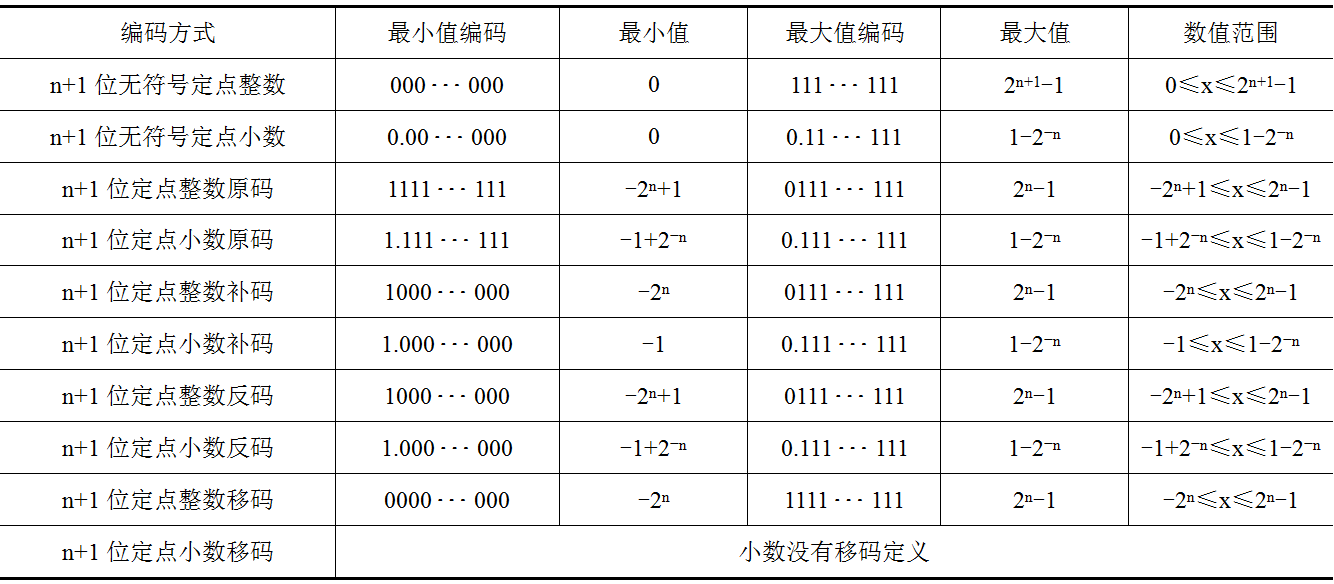
\includegraphics[width=3.46875in,height=1.52083in]{computerassets/0DC0AD3753DD835E184D090930E7A18E.png}
\end{solution}
\question 若x=103,y=-25,则下列表达式采用8位定点补码运算实现时,会发生溢出的是(
)
\par\twoch{x+y}{-x+y}{\textcolor{red}{x-y}}{-x-y}
\begin{solution}这题在考场上时,切不可``盲目''地一步一步去计算补码的加法,因为这两个数字都特别特殊,绝对值之和是128,另外又是采用8位定点补码表示。我们应该立刻联想到8位定点补码表示的数的范围-128\textasciitilde{}127,这样我们只要计算一下四个答案中哪个结果超出这个范围,哪个就溢出了,很明显x-y=128,溢出了。
【总结】这种题目可不是第一次出现在统考卷当中,2009年选择题当中有一题是涉及到浮点数运算的题目,开始的题干给你介绍了一堆关于浮点数加减运算的步骤:对阶、尾数处理、规格化、舍入处理和判断溢出,然后就给了你两个数x和y,让你选出x+y的结果。很多考生看完题干,就立刻开始一步一步按照浮点数运算过程开始来算,那么恭喜你!你中了出题人给你下的套,且不说你能不能算对,就算算对了,在考场这么宝贵的时间里,你花这么多时间来算个选择题,值不值?这个时候我建议大家稍微停那么一两秒钟想想,出题人闲的没事跟你讲那么多运算步骤干什么?为什么不直接说让你用浮点数加法计算x+y的结果呢?这些本该就是你在平时要掌握的。很明显这是在诱导你``误入歧途''。怎么可能在这么紧张的时间内让你去一步步计算呢,所以有时候我们应当从题目中来稍微揣摩一下出题人的意图。这就是在考察我们对一些特殊数字敏不敏感了,我们只要把两个数相加发现超过了浮点数的表示范围,OK那就溢出了,毫不费力。
\end{solution}
\question 某字长为8位的计算机中,已知整型变量x、y的机器数分别为{[}x{]}补=1
1110100,{[}y{]}补=1 0110000。若整型变量z=2*x+y/2,则z的机器数为( )
\par\twoch{\textcolor{red}{1 1000000}}{0 0100100}{1 0101010}{溢出}
\begin{solution}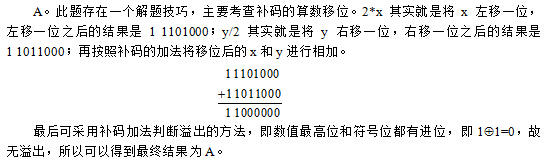
\includegraphics[width=5.73958in,height=1.75000in]{computerassets/f7aa3d33b4082cc7a9bf16eae72bd2a3.jpeg}
\end{solution}
